\section{Sequential Optimization}\label{sec:sequential}

The initial phase of our performance analysis aims to evaluate the baseline matrix multiplication kernel across different compilers (GCC, ICC, and ICX) and optimization levels (from \texttt{-O0} to aggressive flags like \texttt{-O3} and \texttt{-Ofast}). By progressively enabling optimizations and guiding them  towards the fastest implementation reachable, we can systematically identify compiler limitations, expose micro-architectural bottlenecks, and understand how loop transformations, vectorization, and instruction scheduling impact the performances of the algorithm.

\subsection{ICC Optimization Levels}

Although preliminary tests showed comparable baseline performance across GCC, ICX, and ICC, we selected the Intel Classic Compiler (ICC) for our detailed sequential analysis. 

We chose ICC because each progressive optimization flag introduces significant, non-trivial changes to the generated assembly. While ICC is not always the fastest compiler at every intermediate step, its distinct code transformations make it ideal for microarchitectural profiling. Most importantly, as later sections will show, ICC ultimately delivers the highest peak performance for our fully optimized code.

The following subsections examine the effects of increasing ICC's optimization levels by analyzing performance scaling, Intel Advisor rooflines, Valgrind memory traces, and compiler reports.


\paragraph{Interprocedural Optimization.}
In all test cases, the \texttt{-ipo} flag was utilized to enable multi-file Interprocedural Optimization. This is necessary because the matrix multiplication kernel is defined in a separate source file from the \texttt{main.c} driver. Without this flag, the compiler would be unable to perform cross-module optimizations, such as inlining and specialized constant propagation, during the link phase.


%==============================
%-------------O0---------------
%==============================
\subsubsection{No Optimizations (\texttt{-O0})}

We begin by compiling the baseline implementation with the \texttt{-O0} flag, which disables virtually all compiler optimizations. This configuration isolates the raw, intrinsic computational and memory access characteristics of the algorithm without interference from auto-vectorization or loop restructuring. 

\begin{figure}[H]
  \centering
  \noindent
  \makebox[0pt][c]{%
    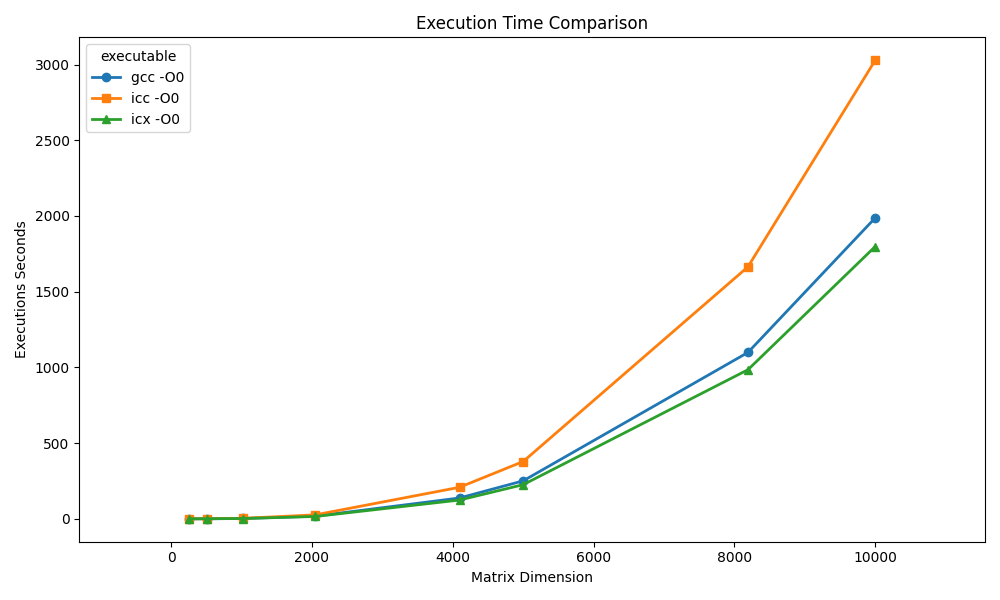
\includegraphics[width=0.6\paperwidth]{Images/all_o0.png}
  }
  \caption{Execution time scaling as a function of matrix size ($n$) at \texttt{-O0}.}
  \label{fig:all_o0}
\end{figure}

\paragraph{Performance Scaling.}
Figure~\ref{fig:all_o0} reports the execution time as a function of matrix size $n$ for the three compilers at \texttt{-O0}. Across all tested input sizes, the scaling behavior strictly follows the expected cubic trend $\mathcal{O}(n^3)$, confirming the theoretical complexity of the algorithm. At this level performance is severely limited, and significant discrepancies observed among the compilers, are not interesting to address, since the generated machine code is a literal, unoptimized translation of the source code.


\paragraph{Intel Advisor and Roofline Analysis.}

The Roofline model (Figure~\ref{fig:icc_o0_roofline}) places the kernel at an extremely low arithmetic intensity ($\approx 0.014$ FLOP/Byte) with a measured performance of merely \textbf{0.66 GFLOPS}. 
Crucially, Advisor indicates that the execution is bottlenecked by the \textbf{Integer Scalar Add Peak} rather than floating-point throughput or memory bandwidth.

\begin{figure}[H]
\centering
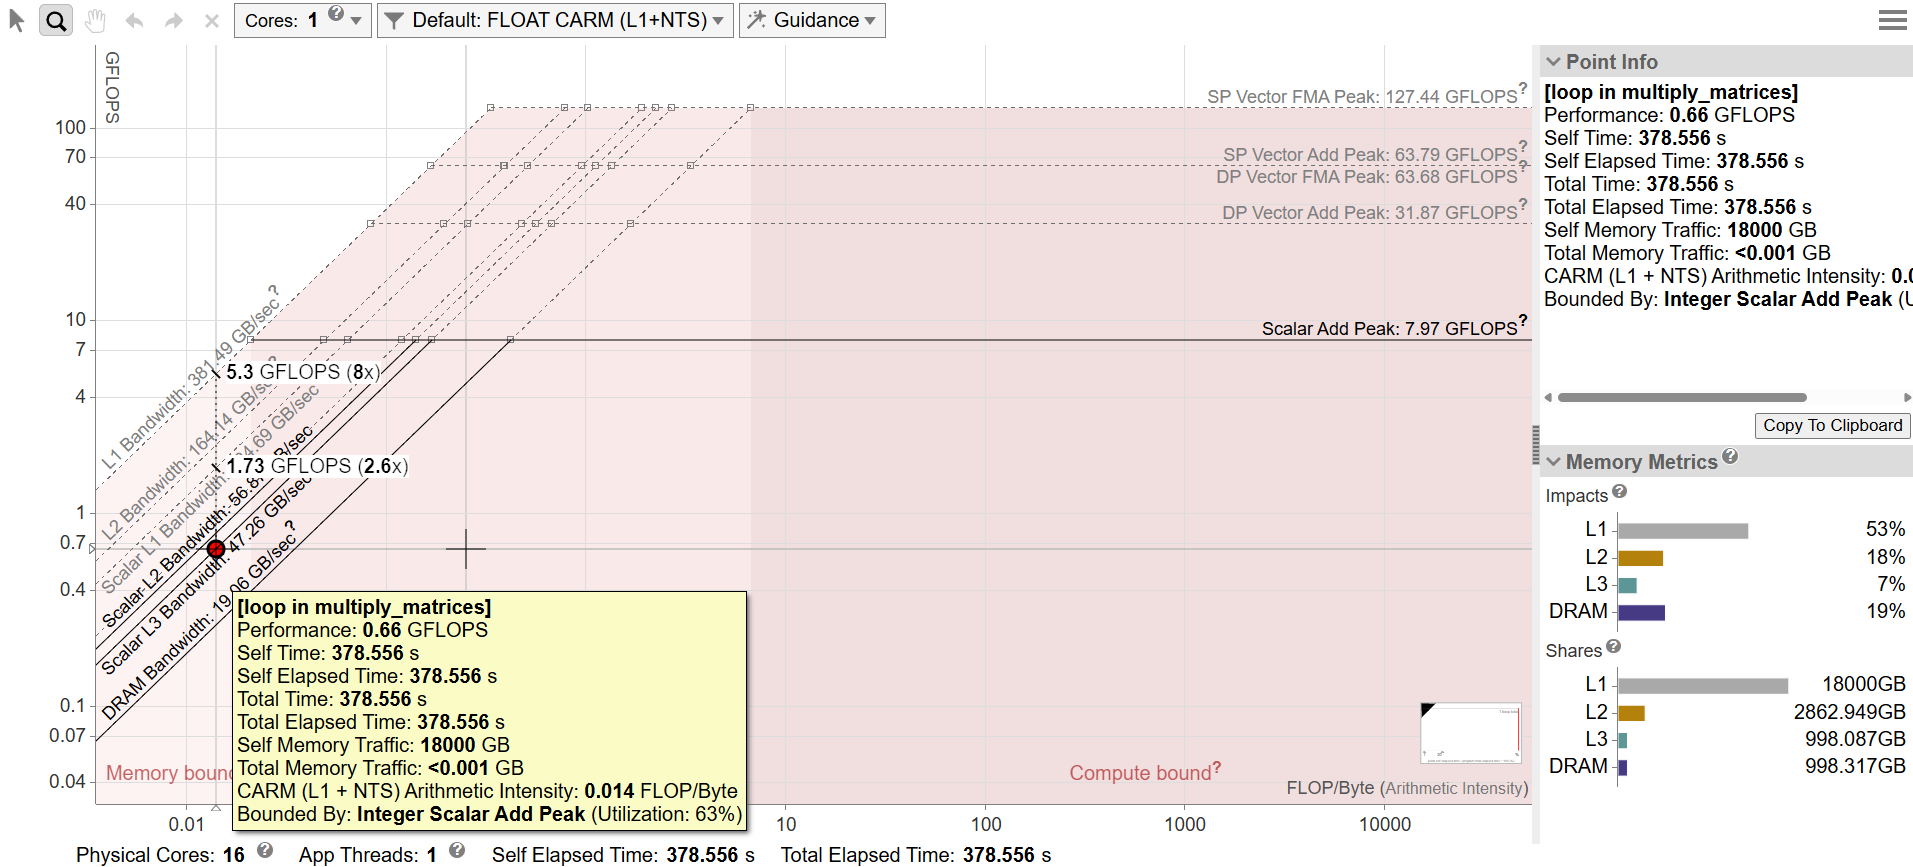
\includegraphics[width=1\textwidth]{Images/icc_o0_roofline.png}
\caption{Intel Advisor Roofline analysis for ICC \texttt{-O0}.}
\label{fig:icc_o0_roofline}
\end{figure}

This massive integer overhead is a direct consequence of the address calculation required for every 2D array access\footnote{The standard 2D array syntax implicitly expands the logical coordinates \texttt{A[i][j]} into a offset \texttt{A[i * n + j]}, requiring a scalar integer multiplication and addition for every single element accessed.}.

Under \texttt{-O0}, the compiler does not perform common subexpression elimination, strength reduction, or loop-invariant code motion. Consequently, these redundant index multiplications and additions are re-evaluated during every single iteration of the innermost loop. Furthermore, the strict lack of register allocation forces the CPU to continuously spill and reload these intermediate address calculations to and from the L1 cache, completely stalling the floating-point pipelines\footnote{This it the main cause of the slow-down, as confirmed by the extremely high number of requests to the L1 cache.}.


\paragraph{Valgrind Cachegrind Analysis.}
The excessive memory traffic caused by the lack of register reuse is confirmed by Valgrind (Figure~\ref{tab:cachegrind_results_o0}). 

\begin{table}[H]
\centering
\caption{Key Valgrind Cachegrind memory profiling metrics for ICC \texttt{-O0}.}
\label{tab:cachegrind_results_o0}
\begin{tabular}{lr}
\toprule
\textbf{Metric} & \textbf{Total Count / Rate} \\
\midrule
Instruction References (I) & \textbf{6,626,402,614,521} \\
Data References (D)        & \textbf{3,000,701,173,012} \\
\midrule
L1 Data Misses             & 31,287,508,170 \\
L1 Data Miss Rate          & 1.0\% \\
\midrule
Last-Level (LL) Misses     & 15,640,639,539 \\
Last-Level (LL) Miss Rate  & 0.2\% \\
\bottomrule
\end{tabular}
\end{table}

The profiling reports approximately 6.6 trillion executed instructions (I refs) alongside 3 trillion data references (D refs). This ratio of roughly 2.2 instructions per data access reflects the massive scalar overhead required simply for loop control and address calculation. 

Despite an enormous cumulative memory traffic footprint ($\approx 18$ TB of L1 interactions), the actual cache miss rates remain relatively low (1.0\% for L1 data, 0.2\% for Last-Level Cache). This confirms that the kernel is not DRAM bandwidth-bound, but rather instruction-bound due to scalar execution.


\paragraph{Compiler Report.}
Finally, the compiler optimization report for \texttt{-O0} confirms the absence of any code transformations. No SIMD instructions are generated (the code relies exclusively on standard scalar x86 instructions), and the nested loops are left entirely intact without unrolling, blocking, or interchange, leading to the severe underutilization of the CPU's computational resources observed in the profiling tools.

%==============================
%-------------O1---------------
%==============================
\subsubsection{Minimal Optimizations (\texttt{-O1})}

The \texttt{-O1} optimization level represents the first step beyond baseline execution, implementing several impacting changes as shown in Figure~\ref{fig:all_o1}.

\begin{figure}[H]
  \centering
  \noindent
  \makebox[0pt][c]{
    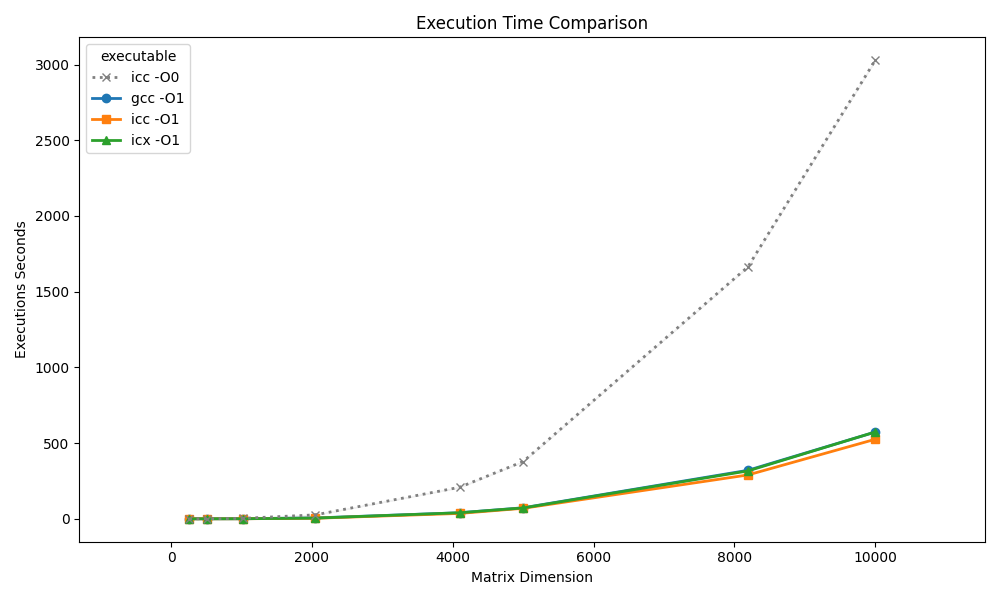
\includegraphics[width=0.6\paperwidth]{Images/all_o1.png}
  }
  \caption{Execution time scaling as a function of matrix size ($n$) at \texttt{-O1}.}
  \label{fig:all_o1}
\end{figure}

At this stage, the compiler enables basic scalar optimizations such as constant folding, dead code elimination, and limited inlining. However, aggressive loop transformations, cache blocking, and automatic vectorization remain inactive. 

The compiler optimization report confirms this behavior, repeatedly issuing the remark: 

\begin{quote}
    \texttt{remark \#15320: routine skipped: loop optimizations disabled}
\end{quote}

This indicates that loop-level optimizations and vectorization passes are not applied under the \texttt{-O1} profile. Consequently, the triple-nested loop is executed in scalar form, failing to exploit the AVX2 SIMD units available on the target architecture. 

Furthermore, the absence of loop restructuring prevents the compiler from improving data locality, leaving the implementation unable to effectively utilize the hardware's caching capabilities.

\paragraph{Intel Advisor Analysis.} 
The Intel Advisor Roofline analysis (Figure~\ref{fig:roofline_o1}) places the kernel in a strictly memory-bound regime. 

\begin{figure}[H]
    \centering
    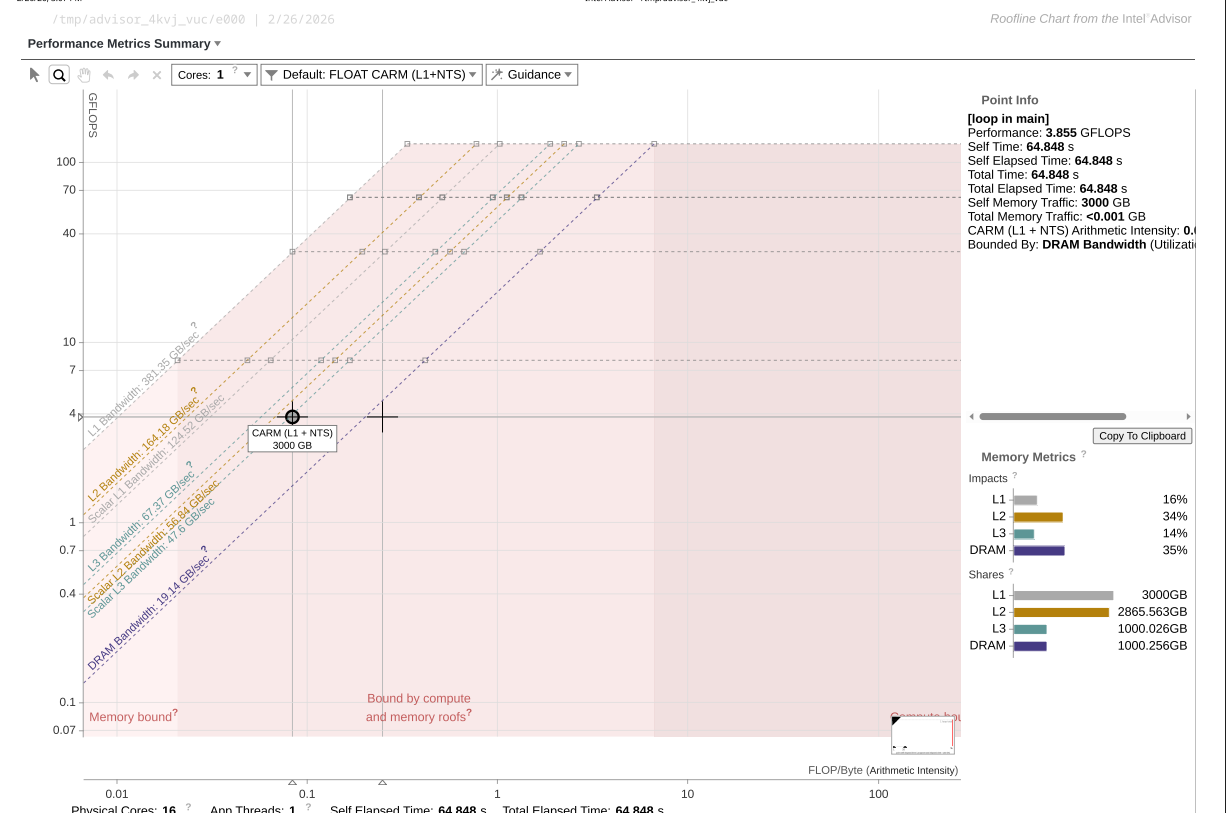
\includegraphics[width=1\textwidth]{Images/icc_o1_roofline.png}
    \caption{Intel Advisor Roofline analysis for ICC \texttt{-O1}.}
    \label{fig:roofline_o1}
\end{figure}

Measured performance reaches \textbf{3.855 GFLOPS}, with an arithmetic intensity of approximately 0.1 FLOP/Byte. Such low intensity indicates that the algorithm performs very few floating-point operations per byte transferred from memory. Execution is thus constrained by memory bandwidth rather than computational throughput, preventing the functional units from reaching their theoretical peak.

The memory hierarchy breakdown further clarifies these performance limitations:

\begin{itemize}
    \item \textbf{Stall Impact:} The dominant stall sources are DRAM (35\%) and L2 (34\%), accounting for nearly 70\% of total execution stalls. This confirms that latency at lower cache levels and main memory significantly limits pipeline utilization.
    \item \textbf{Traffic Distribution:} Memory traffic analysis reports approximately \textbf{3000 GB} of data passing through L1, with the majority propagating to L2 (2865 GB), and nearly 1000 GB reaching L3 and DRAM. This indicates insufficient temporal locality and poor cache residency of the working set.
\end{itemize}

\paragraph{valgrind insight}
Dynamic analysis via Valgrind further corroborates the memory-bound diagnosis. The key metrics for this configuration are summarized in Table~\ref{tab:cachegrind_results_o1}.

\begin{table}[H]
\centering
\caption{Key Valgrind Cachegrind memory profiling metrics for ICC \texttt{-O1} ($n=5000$).}
\label{tab:cachegrind_results_o1}
\begin{tabular}{lr}
\toprule
\textbf{Metric} & \textbf{Total Count / Rate} \\
\midrule
Instruction References (I) & 875,303,318,749 \\
Data References (D)        & 375,101,183,650 \\
\midrule
L1 Data Misses             & 31,309,389,456 \\
L1 Data Miss Rate          & 8.3\% (\textbf{12.5\% Read}) \\
\midrule
Last-Level (LL) Misses     & \textbf{15,640,645,313} \\
Last-Level (LL) Miss Rate  & 1.3\% (6.3\% Read) \\
\bottomrule
\end{tabular}
\end{table}


The L1 data cache exhibits a 12.5\% read miss rate, which is unusually high for high-performance workloads and indicates limited spatial locality within the innermost loop. 
The last-level cache (L3) shows a 6.3\% read miss rate, translating into approximately 15.6 billion accesses to main memory.

Although the overall LL miss rate (1.3\%) appears moderate, the extremely large number of total memory references amplifies the impact of each miss, resulting in substantial DRAM traffic and high latency penalties.

These findings are consistent with the Roofline model and confirm that memory latency and bandwidth represent the primary bottleneck under minimal optimization settings.

\paragraph{Conclusions. }
In summary, the \texttt{-O1} configuration introduces basic scalar optimizations but does not alter the algorithm's fundamental memory access pattern: the combined evidence identifies the kernel as \textbf{bandwidth-bound}.

The triple nested loop remains non-vectorized and untiled, leading to low arithmetic intensity and excessive off-chip memory traffic.



%==============================
%-------------O2---------------
%==============================
\subsubsection{Standard Optimizations (\texttt{-O2})}
The adoption of the \texttt{-O2} optimization level leads to a moderate improvement in performance: at this level, the compiler applies \emph{conservative} optimizations that improve execution speed without "risking" changes to the program's numerical semantics or architectural meaning, such as \textbf{basic auto-vectorization}.

\begin{figure}[H]
\centering
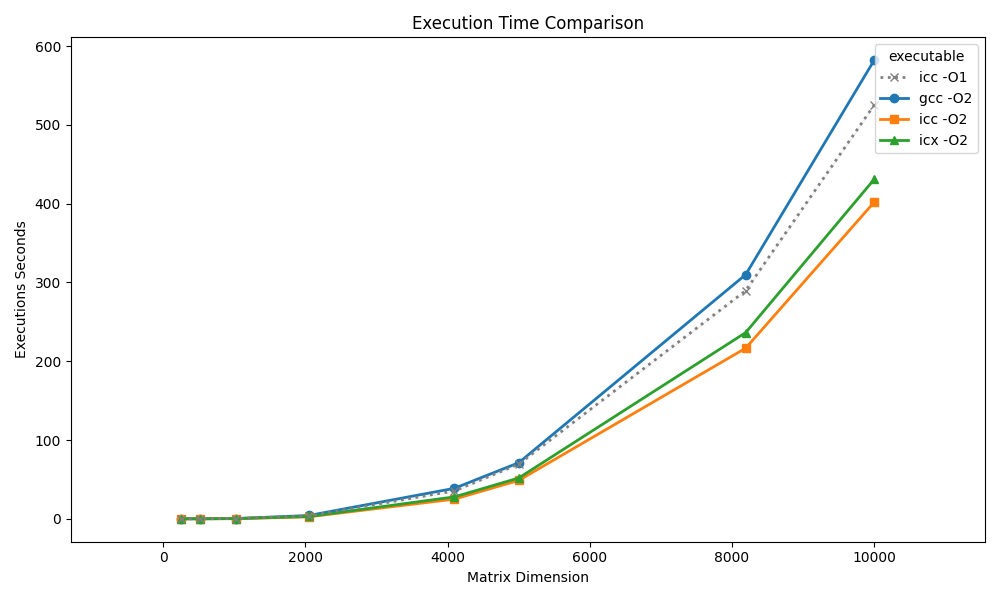
\includegraphics[width=0.8\textwidth]{Images/all_o2.png}
\caption{All compilers -O2 performances compared to ICC -O1}
\label{fig:all_o2}
\end{figure}


\paragraph{Roofline model}
The Roofline model showin in Figure~\ref{fig:icc_o2_roofline} indicates that the working point shifts vertically compared to the \texttt{-O0} configuration, reflecting increased computational throughput at similar arithmetic intensity.
Measured throughput increases to \textbf{6.062 GFLOPS}, corresponding to a 31\% improvement over the previous configuration, and execution time decreases to 49.39 seconds. 

\begin{figure}[H]
\centering
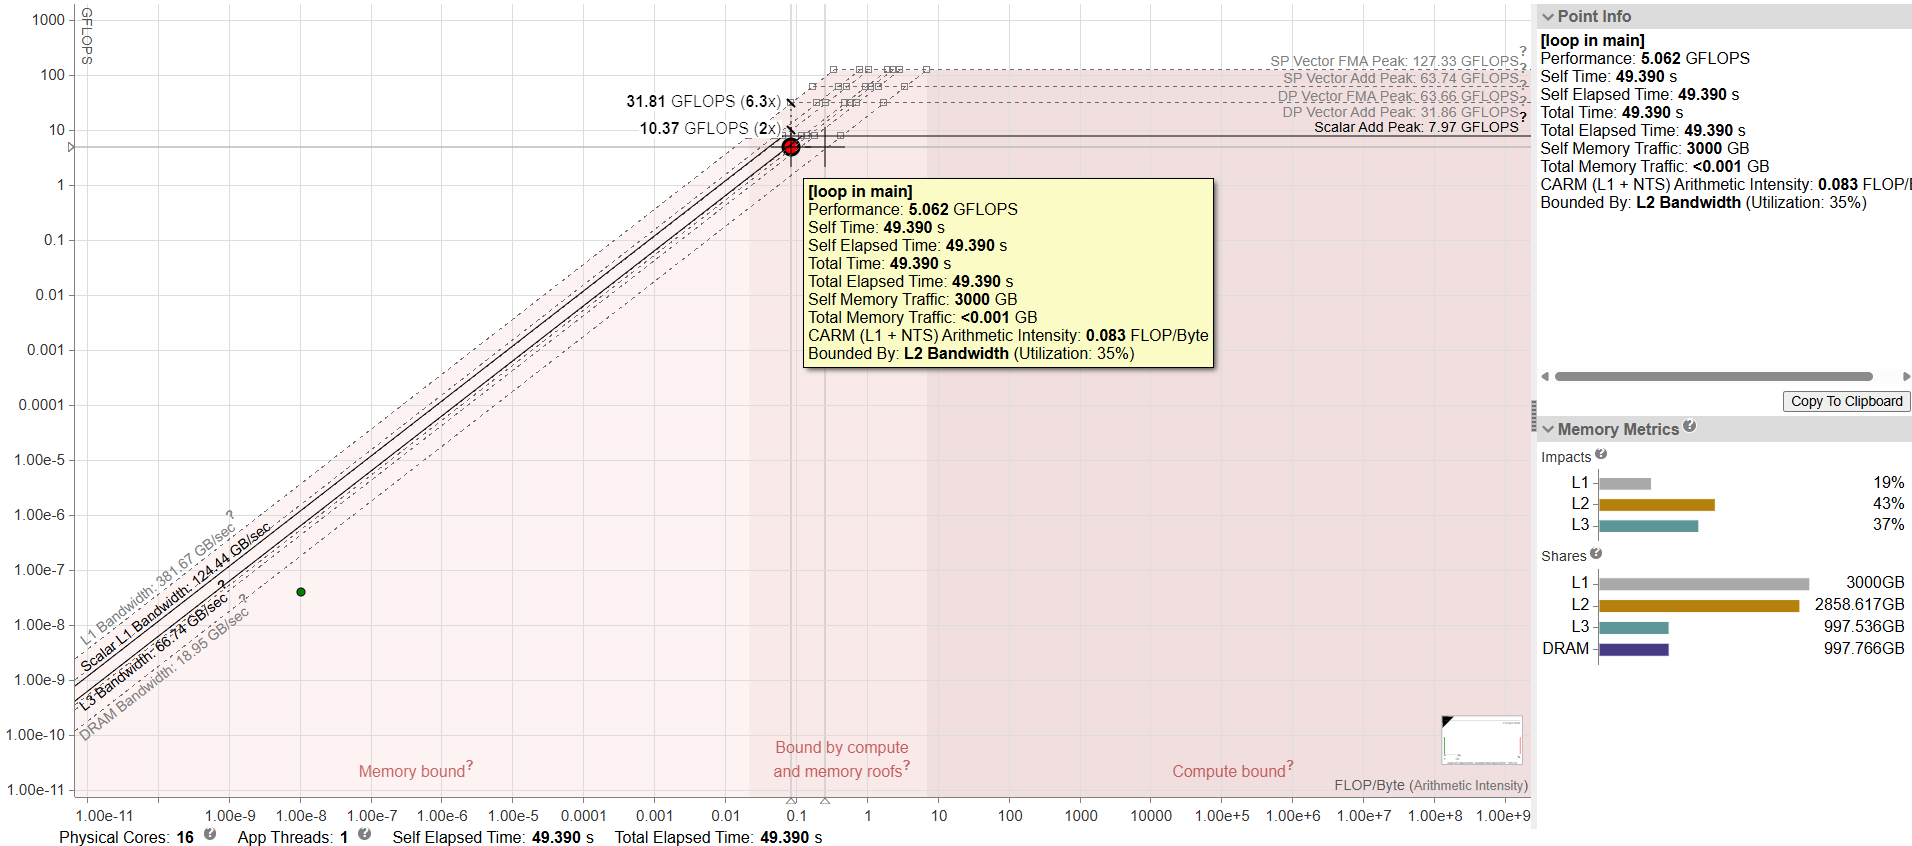
\includegraphics[width=\textwidth]{Images/icc_o2_roofline.png}
\caption{Roofline analysis for ICC -O2.}
\label{fig:icc_o2_roofline}
\end{figure}

The kernel is now bounded by L2 cache bandwidth, as explicitly reported by Advisor (``Bounded by: L2 Bandwidth''). 
This transition suggests that instruction-level inefficiencies have been partially mitigated and that the memory hierarchy has become the dominant constraint.
\paragraph{Valgrind Cachegrind Analysis.}
Dynamic analysis confirms a massive reduction in instruction overhead, though memory pressure has intensified. Key metrics are summarized in Table~\ref{tab:cachegrind_results_o2}.

\begin{table}[H]
\centering
\caption{Key Valgrind Cachegrind metrics for ICC \texttt{-O2}.}
\label{tab:cachegrind_results_o2}
\begin{tabular}{lr}
\toprule
\textbf{Metric} & \textbf{Total Count / Rate} \\
\midrule
Instruction References (I) & 297,143,584,210 \\
Data References (D)        & 187,582,341,902 \\
\midrule
L1 Data Miss Rate          & 16.7\% (25.0\% Read) \\
Last-Level (LL) Miss Rate  & 3.2\% \\
\bottomrule
\end{tabular}
\end{table}

Compared to \texttt{-O1}, the total instruction count fell by nearly 65\% (from 875B to 297B), confirming the efficacy of vectorization. However, the L1 read miss rate has spiked to 25\%. 

This occurs because the faster execution units demand data more aggressively, exposing the locality limitations of the naive $i-k-j$ pattern: the working set exceeds L2 capacity, forcing the stalls observed in the Roofline model.

\newpage
\paragraph{Compiler Report.}
The ICC optimization report confirms that the compiler successfully auto-vectorized the innermost loop, though it utilized a conservative SIMD width.

\begin{lstlisting}[style=CStyle, caption={Simplified ICC Optimization Report for \texttt{-O2}.}]
LOOP BEGIN (i-loop)
    remark #15542: loop was not vectorized: inner loop already vectorized
    LOOP BEGIN (k-loop)
        remark #15542: loop was not vectorized: inner loop already vectorized
        LOOP BEGIN (j-loop)
            remark #15388: aligned access for matrix[i][j] and matrix[k][j]
            remark #15305: vector length 2
            remark #15399: unroll factor set to 4
            remark #15300: LOOP WAS VECTORIZED
        LOOP END
        LOOP BEGIN (j-remainder)
            remark #15335: remainder loop was not vectorized
        LOOP END
    LOOP END
LOOP END
\end{lstlisting}

The report highlights a vector length of 2, indicating \texttt{\textbf{128-bit SIMD}} usage for double-precision operands. This suggests that the compiler is not yet targeting the full 256-bit register's width available on the studied AVX-capable hardware\footnote{The use of 128-bit SIMD instead of 256-bit is a symptom of the code not being fully tuned for the specific target architecture at this optimization level.}. 

Despite this, the unroll factor of 4 and aligned accesses successfully reduced loop-control overhead.


%==============================
%-------------O3---------------
%==============================
\subsubsection{Aggressive Optimizations (\texttt{-O3})}\label{subsec:seq_3}

The adoption of the \texttt{-O3} optimization level produces a dramatic shift in the performance profile of the kernel. At this stage, the compiler goes beyond conservative instruction scheduling and actively restructures the execution pattern to overcome the severe bandwidth bottlenecks caused by poor cache utilization.

\begin{figure}[H]
\centering
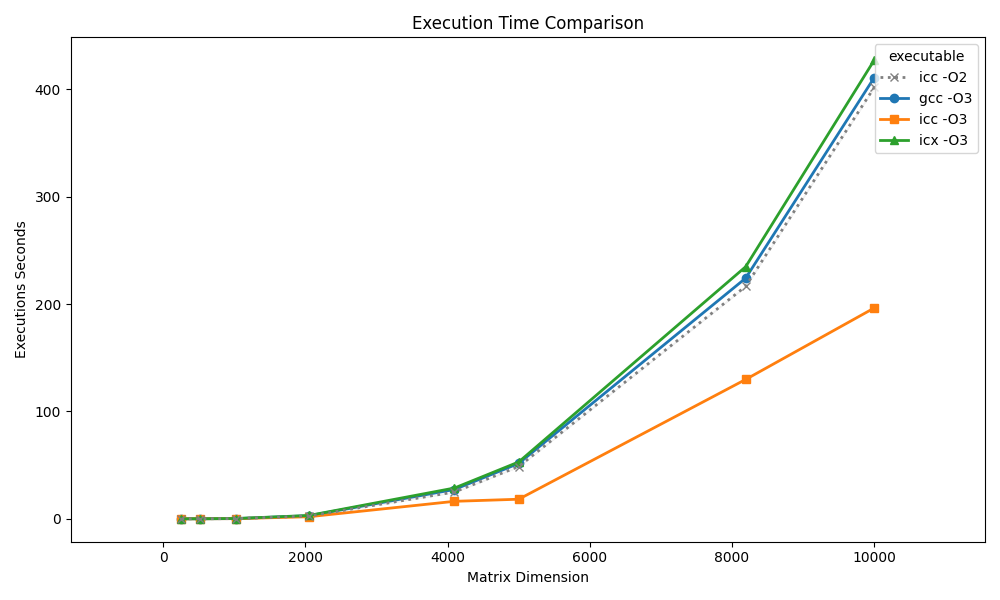
\includegraphics[width=0.8\textwidth]{Images/all_o3.png}
\caption{All compilers -O3 performances compared to ICC -O2}
\label{fig:all_o3}
\end{figure}


\paragraph{Compiler Optimization Report}
The ICC optimization report reveals that the compiler has fundamentally refactored the triple-nested loop into a complex, multi-level structure\footnote{See Appendix~\ref{subsec:tiling} for an in-depth explanation of how the \emph{Tiling Algorithm} works.}.

\begin{lstlisting}[style=CStyle, caption={Refactored ICC Optimization Report for \texttt{-O3}.}]
LOOP BEGIN (i-tile)
    LOOP BEGIN (k-tile)
        LOOP BEGIN (j-tile)
            LOOP BEGIN (i-inner) blocked by 128
                LOOP BEGIN (k-inner) blocked by 128
                    1. LOOP BEGIN (j-peeled)
                    2. LOOP BEGIN (j-vectorized)
                         remark #15388: aligned access
                         remark #15305: vector length 2, unroll factor 4
                         remark #15300: LOOP WAS VECTORIZED
                    3. LOOP BEGIN (j-alternate-alignment)
                    4. LOOP BEGIN (j-remainder)
                         remark #15335: loop not vectorize
                LOOP END
            LOOP END
        LOOP END
    LOOP END
LOOP END
\end{lstlisting}


\paragraph{Intel Advisor Roofline Analysis}
The structural changes translate directly into a massive throughput increase, as shown in the Roofline model (Figure~\ref{fig:icc_O3_roofline}).

\begin{figure}[H]
\centering
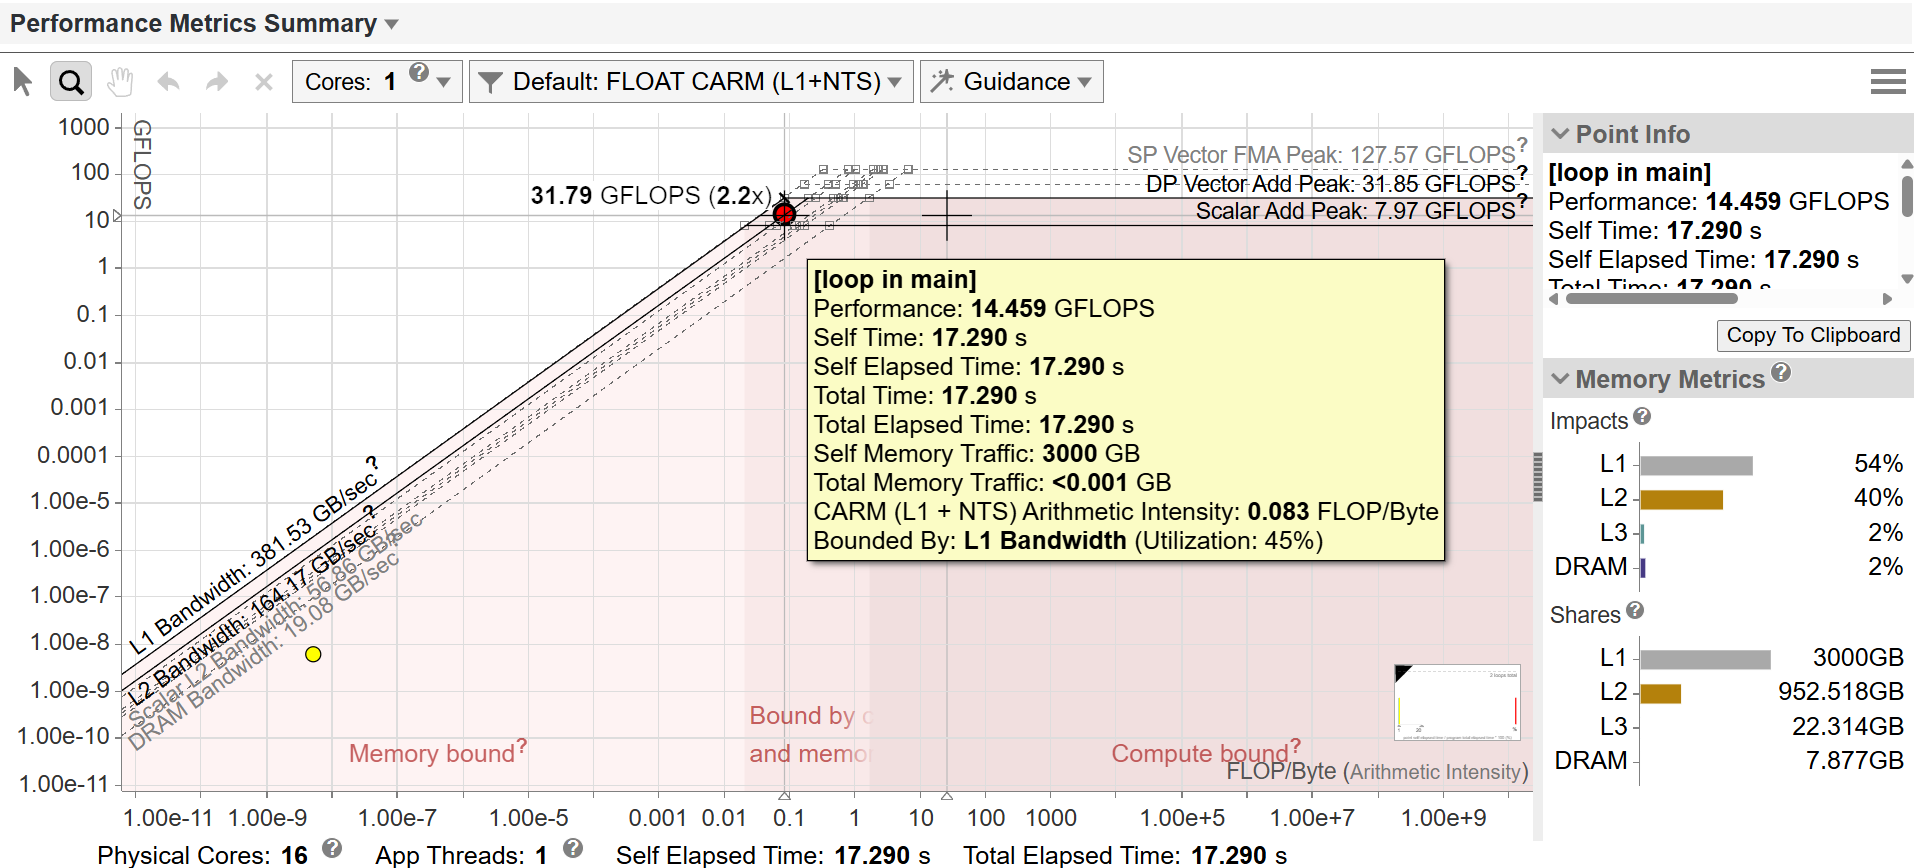
\includegraphics[width=\textwidth]{Images/ICC_O3_Roofline.png}
\caption{Roofline analysis for ICC \texttt{-O3}.}
\label{fig:icc_O3_roofline}
\end{figure}

The kernel achieves a computational throughput of \textbf{14.459 GFLOPS}, a significant uplift from \texttt{-O2} (that performed 6.062 GFLOPS). 

Observe how the \textbf{Arithmetic Intensity (AI)} keep the same value as the previous optimization at $0.083$ FLOP/Byte: this confirms that the performance gain is not due to doing "less memory work" per operation, but rather doing that work much faster by shifting the bottleneck.

The kernel's operational point has exceeded the scalar add peak, moving toward the vector add peak; the bottleneck is now  \textbf{L1 Bandwidth Bound} (saturating 45\% of maximum capacity). 

The decomposition of execution time shows that the L1 cache (54\%) and L2 cache (40\%) are the primary bottlenecks, while DRAM impact is negligible. 

This proves the tiling was successful: the data is now almost entirely encapsulated within the smaller (and faster) caches.

\paragraph{Valgrind Cachegrind Analysis}

The efficacy of the tiling is quantitatively confirmed by the memory profiling in Table~\ref{tab:cachegrind_results_o3}.

\begin{table}[H]
\centering
\caption{Key Valgrind Cachegrind metrics for ICC \texttt{-O3}.}
\label{tab:cachegrind_results_o3}
\begin{tabular}{lr}
\toprule
\textbf{Metric} & \textbf{Total Count / Rate} \\
\midrule
Instruction References (I) & 297,143,584,210 \\
Data References (D)        & 187,582,341,902 \\
\midrule
L1 Data Miss Rate          & \textbf{8.9\%} \\
Last-Level (LL) Miss Rate  & \textbf{0.1\%} \\
\bottomrule
\end{tabular}
\end{table}

The L1D miss rate has dropped significantly to 8.9\%, indicating much better temporal locality. Most importantly, the L3 miss rate is near-zero (0.1\%). This demonstrates that despite the large matrix size, the optimized access pattern ensures that almost no data requests need to traverse the hierarchy to the DRAM. The high degree of data reuse within the primary and secondary caches allows the CPU to sustain much higher GFLOPS by avoiding the high-latency penalty of main memory.

%==============================
%-------------O3 xHost (-DALIGN)---------------
%==============================

\subsection{Compiler(s), to the moon: beyond \texttt{-O3}}

Now that we have studied in-depth the behavior of the compiler given the default optimizations \texttt{-O}, we can further drive the compilation towards even more optimized code by giving even more specific flags to the compilers. 

For brevity, we define a set of these flags simultaneously to evaluate their cumulative impact on the kernel's performance, without explicitly define what is their separate impact on the generated assembly.

\begin{table}[H]
\centering
\begin{threeparttable}
\caption{Advanced compiler optimization flags and their expected effects.}
\label{tab:advanced_flags}
\begin{tabular}{lp{3cm}p{7cm}}
\toprule
\textbf{Flag} & \textbf{Category} & \textbf{Microarchitectural Effect} \\
\midrule
\texttt{-xHost} & Architecture & Instructs the compiler to target the highest instruction set available on the local host\tnote{1}, enabling the widest possible SIMD registers. \\
\midrule
\texttt{-fp-model fast=2} & Floating Point & Enables aggressive floating-point optimizations. It allows for reordering of operations and ignores strict IEEE 754 rules to maximize throughput\tnote{2}. \\
\midrule
\texttt{-fno-alias} & Memory & Asserts that no two pointers point to the same memory location, allowing the compiler to reorder loads and stores without "aliasing" checks. \\
\midrule
\texttt{-inline-level=2} & Inlining & Increases the intensity of function inlining to replace function calls with the actual function body, reducing branch penalties and call overhead. \\
\midrule
\texttt{-unroll-aggressive} & Loop Control & Enables aggressive loop unrolling heuristics, attempting to unroll loops even when the benefit is not immediately obvious to standard logic. \\
\midrule
\texttt{-unroll=4} & Loop Control & Specifically sets the unroll factor to 4, ensuring four iterations are processed as a single block to reduce loop-counter overhead. \\
\bottomrule
\end{tabular}

\begin{tablenotes}
    \footnotesize % This makes the font smaller
    \item[1] \textbf{AVX2} on the tested workstation, as reported in Table~\ref{tab:cpu_specs}.
    \item[2] For this reason, at test time the results of the kernel are explicitly checked to ensure results do not differ from the correct behavior.
\end{tablenotes}
\end{threeparttable}
\end{table}
\paragraph{Refactored Optimization Report.}
The following report summarizes the complex loop transformation strategy achieved with these aggressive flags.


The improvements with respect to the previous iteration are noticeable:

\begin{itemize}
    \item \textbf{Array Refs Replacement:} The compiler avoid the iterative request to obtain \texttt{C[i][j]} at each iteration, and decide to save its value in a register for a way-faster access.

    \item \textbf{Vectorization Width:} While standard \texttt{-O3} utilized a conservative vector length of 2 (128-bit), the addition of \texttt{-xHost} enables \textbf{vector length 4}.
    \item \textbf{Unroll and Jam:} The compiler now implements "Unroll and Jam" by a factor of 4. This technique unrolls the outer loops of a nest and fuses the resulting bodies, which significantly improves register reuse and ensure  a better use of the caches hierarchy\footnote{The exact steps implemented, along with the motivations, are explained in Appendix~\ref{subsec:unroll_jam}.}.
    \item \textbf{Vectorized Remainders:} The compiler now successfully \textbf{vectorizes the remainder loops}. This ensures that performance does not drop sharply at the boundaries of the matrix tiles.
\end{itemize}

\newpage
\begin{lstlisting}[style=CStyle, caption={Simplified ICC Report:\texttt{-O3 -xHost}.}]
LOOP BEGIN (i - tile )
    LOOP BEGIN (k - tile )
        LOOP BEGIN (j - tile )
            remark #25440: unrolled and jammed by 4 (pre-vector)    
            LOOP BEGIN (i - inner ) blocked by 128
                LOOP BEGIN (k - inner ) blocked by 128
                    LOOP BEGIN (j-vectorized) blocked by 128
                        remark #15289: vectorization support: unaligned access 
                        remark #15295: vectorization support: vector length 4
                        remark #15297: vectorization support: unroll factor set to 4
                        remark #15298: LOOP WAS VECTORIZED
                        remark #15300: Number of Array Refs Scalar Replaced In Loop
                    LOOP END
                    LOOP BEGIN (j-remainder)
                        remark #15301: REMAINDER LOOP WAS VECTORIZED
                        remark #15302: Number of Array Refs Scalar Replaced In Loop
                    LOOP END
                LOOP END
            LOOP END
        LOOP END
    LOOP END
LOOP END
\end{lstlisting}


\paragraph{Intel Advisor Roofline Analysis}

The impact of the \texttt{-xHost} flag is clearly visible in the transition to AVX2 execution. The kernel now achieves a computational throughput of \textbf{29.463 GFLOPS}. This is approximately double the performance of the standard \texttt{-O3} configuration, which reached 14.459 GFLOPS.

\begin{figure}[H]
\centering
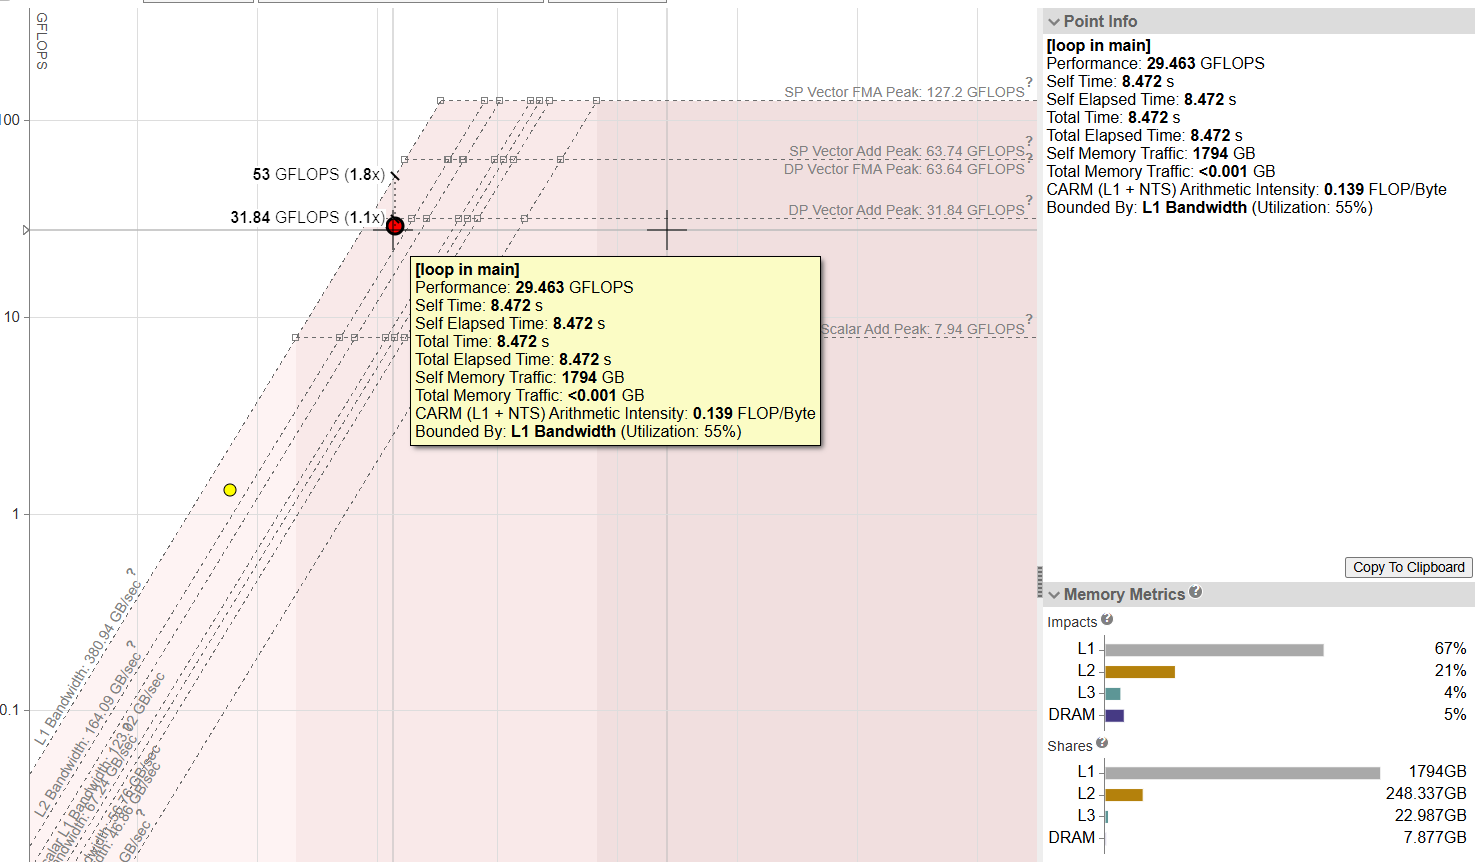
\includegraphics[width=1\textwidth]{Images/icc_better_roofline.png}
\caption{Roofline analysis for ICC \texttt{-O3 -Xhost etc...}.}
\label{fig:icc_better_roofline}
\end{figure}

The operational point on the Roofline model confirms this architectural shift, as the kernel now sits just under the DP Vector Add Peak (31.84 GFLOPS).

\paragraph{Performance comparison}

Lastly, we compare the performance of ICC against ICX\footnote{The ICX report indicates the same optimizations, with the exception that block sizes are $64 \times 64 \times 64$, whereas ICC utilizes $128 \times 128 \times 128$.} across a significantly broader domain of matrix sizes.

\begin{figure}[H]
\centering
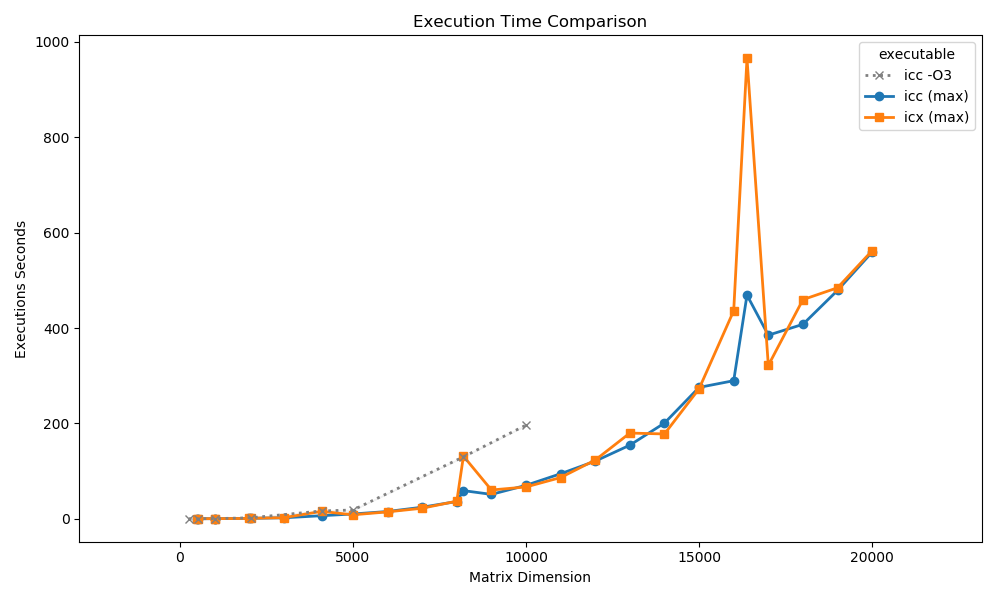
\includegraphics[width=0.8\textwidth]{Images/icc_icx_max.png}
\caption{Performance comparison of ICC and ICX with the advanced flags.}
\label{fig:icc_icx_better_comparison}
\end{figure}

It is immediately apparent that both highly optimized executables suffer a significant performance degradation when the matrix dimension $n$ is a power of 2 (e.g.,$n=4096$, $n=8192$, $n=16384$). 
In contrast, performance remains consistently high and scales more predictably when $n$ does not align with these boundaries.
This specific bottleneck is well motivated in the in-depth explanation in Appendix~\ref{subsec:caching}.

Nonetheless, we will also attempt once again to obtain another improvement: as noted in the optimization report, the main loop body still notify unaligned accesses, which limits the efficiency of the SIMD operations.

\subsubsection{A little price to pay for salvation? \texttt{-DALIGN}}
Note that a standard cache line is 64 bytes, which perfectly accommodates 8 double-precision (8-byte) values. 
When the matrix dimension $n$ (in particular the row's lenght) is not a multiple of 8, the compiler must generate "peeled" and "remainder" loops to handle those edge cases\footnote{Misalignment can also occur if the starting memory address is not aligned with the cache line boundary, but this is easily avoided by calling \texttt{posix\_memalign(ptr, 64, tot\_bytes)} at runtime.}.

By enabling the \texttt{-DALIGN} flag, we explicitly augment the matrix size from $n \times n$ to $n' \times n'$, where $n'$ is the smallest multiple of 8 greater than or equal to $n$.


The "overflow" cells in this padding area are initialized to zero to ensure they do not affect the mathematical results of the matrix multiplication (as explained in Appendix~\ref{subsec:padding}).

\paragraph{Practical Advantages.}

This approach, \textbf{while requiring slightly more memory}, provides several advantages:

\begin{itemize}
\item \textbf{Cache Line Alignment:} 
It is explicitly ensured by the code itself, without relying on the compiler's optimizations.

\item \textbf{Loop Simplification:} Because every row is now also a multiple of the register's capacity (4 doubles), the compiler no longer needs to generate auxiliary loops.

\item \textbf{SIMD Efficiency:} The hardware can perform 256-bit loads and stores at peak speed, as there is no longer a risk of a single vector instruction spanning across two different cache lines (nor incomplete register, that must be explicitly masked with zeros).
\end{itemize}


\paragraph{Compilation report}
The report produced by ICC clearly show a shortened, simplified version of the previous iteration\footnote{The  report from ICX showed once again how the only difference was in the choice of the block size, as before $64 \times 64 \times 64$.}.


\begin{lstlisting}[style=CStyle, caption={Optimization report of ICC with \texttt{-O3 -xHost -DALIGN}.}]
LOOP BEGIN (i-tile)
    LOOP BEGIN (k-tile)
        LOOP BEGIN (j-tile)
            remark #25440: unrolled and jammed by 4 (pre-vector)    
            LOOP BEGIN (i-inner) blocked by 125
                LOOP BEGIN (k-inner) blocked by 125
                    LOOP BEGIN (j-vectorized) blocked by 128
                        remark #15388: vectorization support: reference C[i][j] has aligned access
                        remark #15388: vectorization support: reference B[k][j] has aligned access
                        remark #15305: vectorization support: vector length 4
                        remark #15399: vectorization support: unroll factor set to 4
                        remark #15300: LOOP WAS VECTORIZED
                    LOOP END
                    LOOP BEGIN (j - remainder )
                        remark #15301: REMAINDER LOOP WAS VECTORIZED
                    LOOP END
                LOOP END
            LOOP END
        LOOP END
    LOOP END
LOOP END
\end{lstlisting}

\paragraph{Performance}

Figure~\ref{fig:icc_icx_aligned_comparison} demonstrates that even if \texttt{-DALIGN} successfully lowers execution times, matrices with dimensions power-of-two (and neighboring values) remain a major bottleneck.

\begin{figure}[H]
\centering
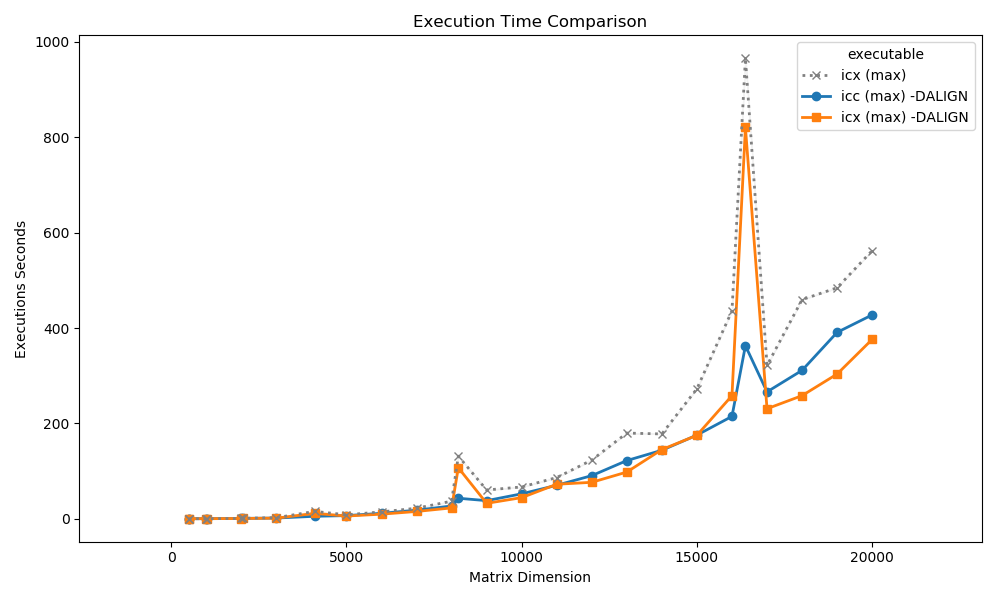
\includegraphics[width=0.8\textwidth]{Images/icc_icx_aligned.png}
\caption{Performance comparison of ICC and ICX with the advanced flags and -DALIGN.}
\label{fig:icc_icx_aligned_comparison}
\end{figure}

ICX achieves the best overall performance in standard cases but suffers the most extreme penalties at problematic dimensions. In contrast, ICC is slightly slower on average but far more stable, handling worst-case scenarios with much greater consistency.

Now we are equipped to  better understand the problem with those last implementations.


%==============================
%-------------EXPLICIT TILING ---------------
%==============================
\subsection{Compiler's limitation, and how to bypass them}

The compiler’s strategy of partitioning the iteration space into blocks $128 \times 128 \times 128$, supplemented by a 4-way unroll-and-jam transformation, is explicitly engineered to maximize the utilization of the  memory hierarchy. 

With those implementation choices, a single $128 \times 128$ tile of requires 128 KB of memory. While this exceeds the 48 KB L1D cache capacity, the \emph{unroll-and-jam} allow for sub-tiles to stay in L1D, while the full $128 \times 128$ block fits inside the L2 cache (1.25 MB per core). 

However, this hardware-specific optimization counld falls short in practice, due to a fundamental limitation in the cache implementation (Behavioral details of the Associative Caches are discussed in Appendix~\ref{subsec:caching}). 

\subsubsection{Cache Collisions in Matrix Traversal}
For simplicity, we consider an aligned matrix implementation with cache-line padding (i.e., the starting pointer is cache-aligned, and the matrix content is perfectly bounded by cache lines): under those constrains, we can find the worst-case scenario of cache trashing.

When iterating through a matrix column, the CPU accesses addresses separated by the length of an entire matrix row. If this row length in memory exactly matches the distance between \emph{cache sets}, the first element of every row will map to the exact same, causing severe cache thrashing by evicting one of the already-allocated cache lines\footnote{Usually the cache eviction follows a Least-Recently-Used (LRU) replacement policy, hence will be removed the cache line first addressed.}.

For a cache with a power-of-two number of sets, addresses map to the same set if they are separated by exactly $2^{(\text{Set bits} + \text{Offset bits})}$ bytes. For a matrix of double-precision floating-point numbers (\texttt{sizeof(double)} $= 8$ bytes), the required row length to force a collision is:
$$ \text{Row Length} = \frac{2^{(\text{Set bits} + \text{Offset bits})}}{8} \text{ elements} $$

Based on the hardware specifications in Table~\ref{tab:cache_partitioning}, we can calculate the exact matrix dimensions that trigger these set collisions:

\begin{itemize}
    \item \textbf{L1 Cache Collision:} 
    The L1 cache uses 6 Offset bits and 6 Set bits.
    $$ \text{L1 Distance} = 2^{(6 + 6)} = 2^{12} \text{ bytes} = 4096 \text{ bytes} $$
    $$ \text{L1 Row Length} = \frac{4096}{8} = 512 \text{ elements} $$
    If the matrix has exactly 512 columns (or a multiple of it), the first element of every row maps to the same L1 set. Since the L1 is 12-way associative, reading just 13 rows in a column will completely fill the set and force an eviction of the first row (as observed in Figure~\ref{fig:icc_icx_aligned_comparison}).

    \item \textbf{L2 Cache Collision:}
    The L2 cache uses 6 Offset bits and 11 Set bits.
    $$ \text{L2 Distance} = 2^{(11 + 6)} = 2^{17} \text{ bytes} = 131,072 \text{ bytes} $$
    $$ \text{L2 Row Length} = \frac{131072}{8} = 16,384 \text{ elements} $$
    If the matrix has exactly 16,384 columns, column-major traversal will rapidly thrash the 10-way associative L2 cache.
\end{itemize}

\paragraph{Quantitative comparison}
This limitation can be verified by the in-depth study we completed by using Intel Advisor on the same ICX build (\texttt{-O3 -xHost -DALIGN}), testing both $N = 4096$ and $N=5000$.

\begin{figure}[H]
\centering
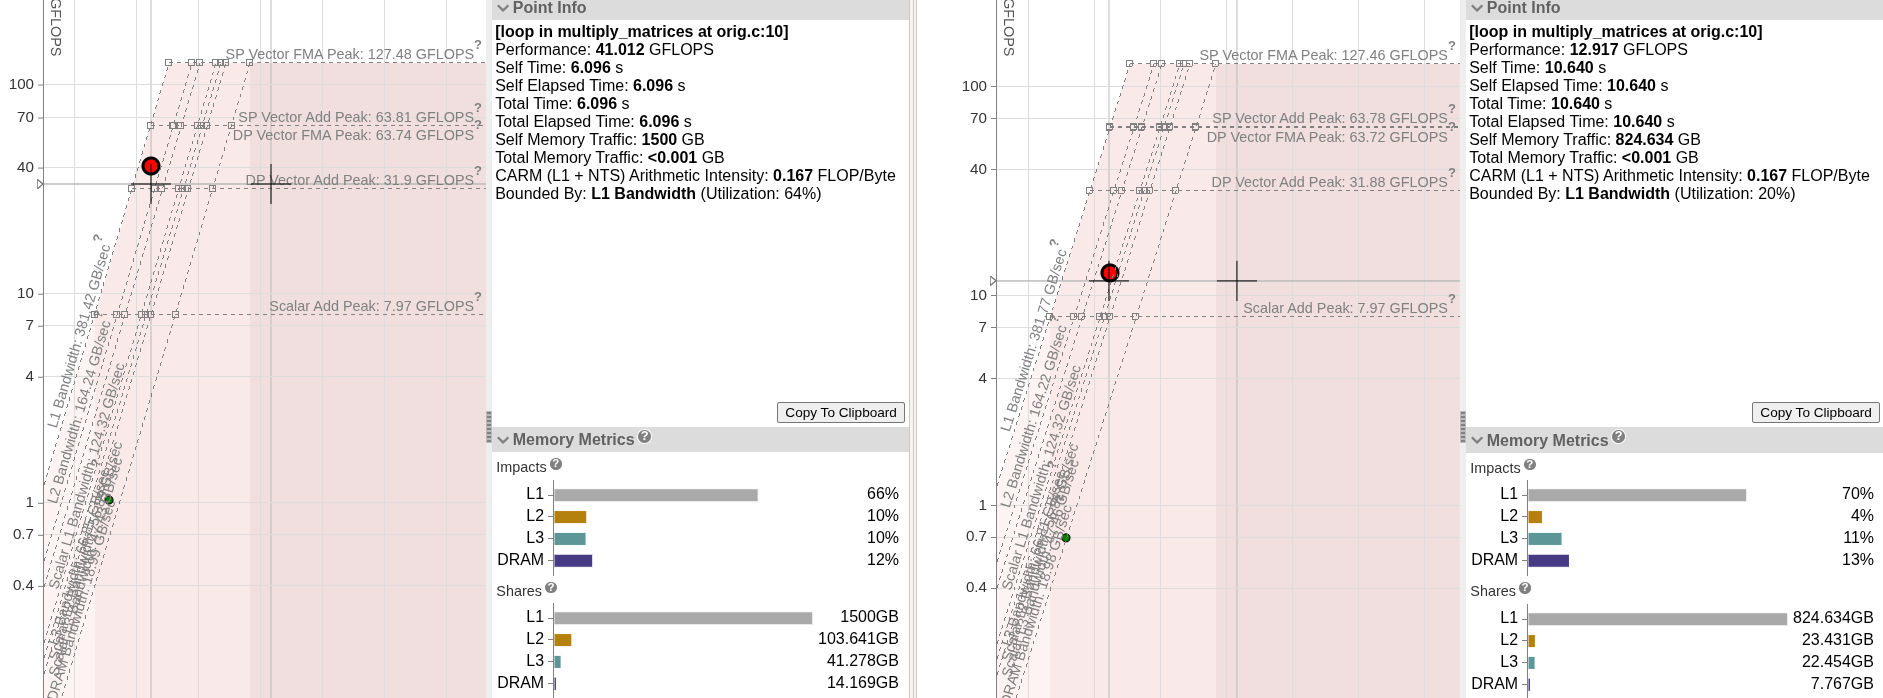
\includegraphics[width=1\textwidth]{Images/icx_4096_vs_5000.png}
\caption{Roofline model of \texttt{ICX -O3 -xHost -DALIGN} on \texttt{n=5000} and \texttt{n=4096}}
\label{fig:icc_icx_aligned_roofline_comparison}
\end{figure}


The highlighted bottlenecks are in both cases the L1, but we can clearly see a difference in their bandwidth utilization and overall performance impact. For the bigger matrix ($N=5000$), the L1 cache is utilized efficiently at 64\% of its peak bandwidth, allowing a performance of \textbf{41.01 GFLOPS}.

In contrast, the problematic one ($N=4096$) suffers a drop  to just \textbf{12.91 GFLOPS}. 

Despite executing fewer total mathematical operations (due to the smaller size), its L1 bandwidth utilization drops to a mere 20\%: this low utilization indicates that the CPU pipeline is heavily stalled waiting for data due to continuous cache conflict evictions (thrashing).



\subsubsection{Cache-Aware Solutions, to Dimension-Dependent Thrashing}

The cache thrashing problem  maximized by power-of-two matrices can be mitigated using three (alternative or complementary) strategies:

\begin{itemize}
    \item \textbf{Memory Padding:} extending each matrix row with a adequate number of cells (zeroed or inaccessible).
    By artificially forcing the row length to a non-power-of-two size\footnote{is possible to compute a runtime a heuristic matrix size that minimize problem, but for brevity purposes we will not explore those solutions.}, the memory addresses are staggered. 
    This naturally shift the column elements across different cache sets rather than concentrating them into the same one. 
    
    We discard this solution because it wastes significant memory space. Furthermore, it assumes we have full control over the original matrices allocations, which is rarely true in real-case scenarios.\footnote{Note that this differs from the minor cache-line alignment padding introduced earlier; padding to break L1 set collisions requires way larger, system-dependent offsets.}

    \item \textbf{Compile-Time Constant Dimensions:} The second solution relies on aggressive compiler optimization. When the matrix dimension $N$ is provided as a constant at compile time, the compiler can further mitigate the effect by using \emph{register blocking} (scalar replacement). Instead of repeatedly fetching conflicting addresses from the L1 cache, the compiler loads the active working set directly into the CPU's vector registers and holds them there throughout the inner loop's execution. 
    
    As shown in Table~\ref{tab:results_placeholder}, the compiler's knowledge partially mitigate the problem, but without completely removing it.

    \begin{table}[H]
    \centering
    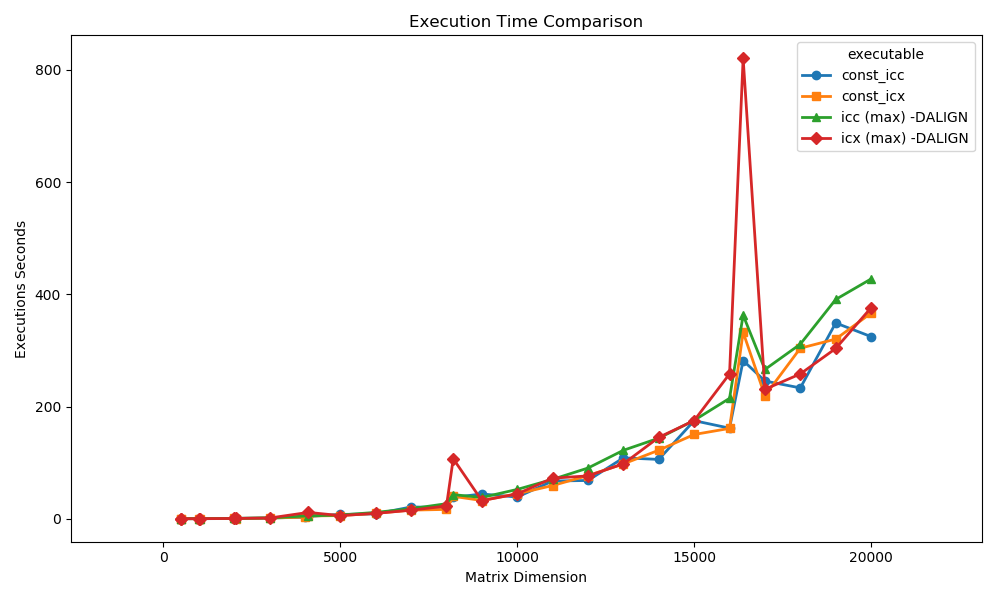
\includegraphics[width=0.8\textwidth]{Images/icc_icx_const.png}
    \caption{Performance comparison demonstrating the furhter dumping of cache thrashing spikes when $N$ is known at compilation time.}
    \label{tab:results_placeholder}
    \end{table}

    \item \textbf{Data Packing (Auxiliary Buffers):} The Last solution proposed is a technique widely employed by high-end optimization libraries such as \texttt{\texttt{OpenBLAS}}, whose detailed breakdown is provided in Appendix~\ref{subsec:openblas}. 
    
    The core idea is to explicitly allocate auxiliary memory buffers and manually copy the active tiles from matrices A and B into these buffers before computing them. Because these temporary matrices are strictly contiguous, they map cleanly across all available cache sets, completely bypassing the original column-stride layout. If implemented correctly and with suitable tile's dimensions, the time used to copy the tiles  will be largely repaid by the performance gains.
\end{itemize}

In the following section, we will present a custom, ad-hoc implementation that applies this packing strategy.


%==============================
%-------------openBlas-like implementation ---------------
%==============================
\subsection{BLAS-like implementation}
Since the attempts to drive the compiler toward the best possible optimization failed, the last chance we have is to explicilty use \texttt{\textbf{AVX intrinsics}} to leverage the CPU's extended registers.

While the low-level implementation motivation are extensively explained in Appendix~\ref{subsec:openblas}, some tinkering with the code was needed to make it work with our use case. 

\subsubsection{Kernel $4\times8$}
In particular, the heart of the  algorithm is the \emph{kernel}, capable to work on multiple cells at the same time; we had to explicitly define it\footnote{In high-end libraries is directly written in Assembly or is written in a source code already "expanded" (i.e. with explicit unrolling, jamming, ...) by scripts that manages all edge-cases and hardware-dependent implementations.}.

\begin{lstlisting}[style=CStyle, caption={Kernel $4\times8$ doubles implementation},label={blas_like_code}]
static inline void kernel_4x8(int n, double (*C)[n], 
                              const double packedA_panel[KC][4], 
                              const double packedB_panel[KC][8], 
                              int kc, int i0, int j0) {
    __m256d c[4][2]; 
    #pragma unroll(4)
    for (int i = 0; i < 4; i++) { // Initialize accumulators
        c[i][0] = _mm256_setzero_pd();
        c[i][1] = _mm256_setzero_pd();
    }
    for (int p = 0; p < kc; p++) { //iterate over kc
        __m256d b0 = _mm256_load_pd(&packedB_panel[p][0]);
        __m256d b1 = _mm256_load_pd(&packedB_panel[p][4]);

        #pragma unroll(4)
        for (int i = 0; i < 4; i++) {
            __m256d a = _mm256_broadcast_sd(&packedA_panel[p][i]);
            c[i][0] = _mm256_fmadd_pd(a, b0, c[i][0]);
            c[i][1] = _mm256_fmadd_pd(a, b1, c[i][1]);
        }
    }
    #pragma unroll(4)
    for (int i = 0; i < 4; i++) {  // Update result matrix C
        __m256d orig0 = _mm256_load_pd(&C[i0 + i][j0 + 0]);
        __m256d orig1 = _mm256_load_pd(&C[i0 + i][j0 + 4]);
        _mm256_store_pd(&C[i0 + i][j0 + 0], _mm256_add_pd(orig0, c[i][0]));
        _mm256_store_pd(&C[i0 + i][j0 + 4], _mm256_add_pd(orig1, c[i][1]));
    }
}
\end{lstlisting}

 It calculates a $4 \times 8$ block of the destination matrix $C$ by multiplying a packed $4 \times kc$ panel of $A$ with a packed $kc \times 8$ panel of $B$. 

\paragraph{Optimization details}
This kernel is designed to fully utilize the capabilities of the AVX2 instruction set, which guarantees \texttt{\textbf{$16 \times$ 256-bit YMM}} registers. 

The kernel at any time keep a $4 \times 2$ array of \texttt{\_\_m256d} vectors. Since each vector holds four double-precision floating-point numbers, the 8 registers stores the 32 elements of the $4 \times 8$ target block of $C$.

By keeping the 8 accumulator registers, 2 registers for $B$, and 1 register for $A$ strictly in the CPU hardware, this kernel uses exactly 11 out of the 16 available \texttt{YMM} registers. This deliberate $4 \times 8$ sizing guarantees that all intermediate calculations occur without any costly "register spilling" to the L1 cache. 

After the iteration along the hidden dimension kc, the accumulated results are loaded, added to the original unaligned $C$ memory locations, and written back.

\paragraph{AVX Intrinsics Reference}
To achieve this low-level control, the kernel relies on Intel Intrinsic functions, which map directly to specific assembly instructions.

\begin{table}[H]
\centering
\caption{AVX2 Intrinsics used in the $4 \times 8$ kernel.}
\label{tab:avx_intrinsics}
\begin{tabular}{lp{10cm}}
\toprule
\textbf{Intrinsic Function} & \textbf{Hardware Operation} \\
\midrule
\texttt{\_\_m256d} & The underlying data type representing a 256-bit \texttt{YMM} register, that can holds 4 double-precision numbers. \\
\midrule
\texttt{\_mm256\_setzero\_pd()} & Returns a 256-bit vector with all bits set to zero.\\
\midrule
\texttt{\_mm256\_load\_pd(ptr)} & Loads 4 packed double-precision values from memory into a vector.\\
\midrule
\texttt{\_mm256\_broadcast\_sd(ptr)} & Loads a single double-precision value from memory and duplicates (broadcasts) it across all 4 elements of the destination vector. \\
\midrule
\texttt{\_mm256\_fmadd\_pd(a, b, c)} & Performs a Fused Multiply-Add operation. It computes $(a \times b) + c$ for all 4 packed elements simultaneously, maintaining infinite intermediate precision before rounding. \\
\midrule
\texttt{\_mm256\_add\_pd(a, b)} & Performs a standard element-wise addition of two 256-bit vectors containing double-precision values. \\
\midrule
\texttt{\_mm256\_storeu\_pd(ptr, a)} & Stores 4 double-precision values from a vector into a  memory location.\\
\bottomrule
\end{tabular}
\end{table}

\paragraph{Hyperparameter tuning}
The algorithm requires tuning the tiling dimensions \texttt{\textbf{MC, NC}}, and \texttt{\textbf{KC}}. The static kernel size ($N_R = 8$, $M_R = 4$), along with the simplification implemented imposes strict alignment constraints: $K_C$ and $N_C$ must be multiples of 8, and $M_C$ must be a multiple of 4.

While theoretical upper bounds can be calculated based on the hardware cache limits in Table~\ref{tab:cache_partitioning}, dictates that the dimensions must be carefully balanced to prevent L2 cache eviction\footnote{The constraints are that: (1) $K_C \times N_R$ elements must fit within the L1 cache; (2) $M_C \times K_C$ elements must fit within the L2 cache, and (3) $N_C \times K_C$ elements must fit within the L3 cache.}.

In the end, rather than relying solely on theoretical maximums, we conducted an empirical search over various block-sized configurations, finding the best-performing tuple defined by $$\texttt{\(\textbf{MC=256, NC=512, KC=256}\)}$$

\paragraph{What is missing from the original}

Compared to the official \texttt{OpenBLAS} library, our custom implementation performs a little worse (ee Figure~\ref{fig:openblas_vs_blas_roofline}). This is mainly caused by the fact that the highly optimized \texttt{OpenBLAS} architecture utilizes a $6 \times 8$ kernel (that obviously performs better, since it uses more registers). 

However, as detailed in Appendix~\ref{subsec:openblas}, by using a $6 \times 8$ kernel significant implementation hazards arises, since the kernel must also work on the  edge of the matrices.

By opting for a $4 \times 8$ kernel and by constraining the use of our \texttt{-DALIGN} padding strategy, we avoid altogether these complications. Because our matrices are explicitly padded to ensure their dimension $n'$ is always a multiple of 8, the $4 \times 8$ kernel inherently divides the iteration space evenly.

\subsubsection{Performances evaluation}
To verify the effectiveness of our implementation we directly compare it with the original one from \texttt{openBLAS}, using once again Intel Advisor.

\begin{figure}[H]
\centering
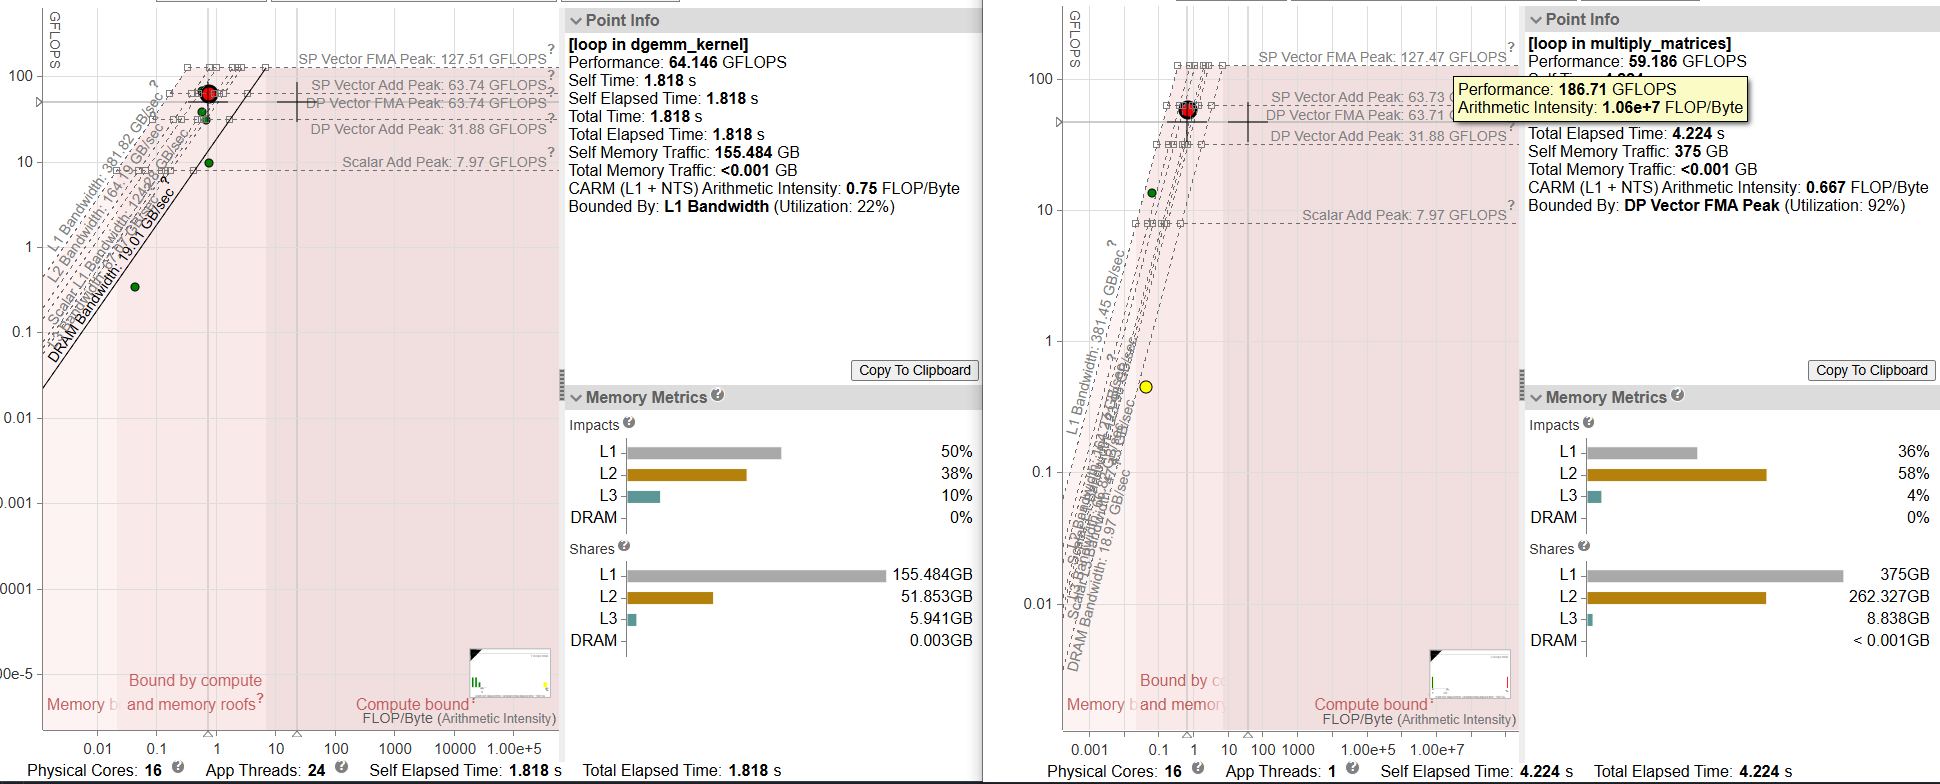
\includegraphics[width=1\textwidth]{Images/openblas_vs_blas_roofline.png}
\caption{Roofline comparison between the original \texttt{OpenBLAS} (left) and our custom implementation (right).}
\label{fig:openblas_vs_blas_roofline}
\end{figure}

As expected, the original \texttt{OpenBLAS} implementation achieves a slightly higher throughput of \textbf{64.146 GFLOPS}. It is classified as bounded by \textbf{L1 Bandwidth}, saturating it with a higher Arithmetic Intensity of $0.75$ FLOP/Byte; there is very little room left for optimization on the machine.

On the other hand, our custom $4 \times 8$ implementation is bounded by the \textbf{DP Vector FMA Peak}, reaching \textbf{59.186 GFLOPS}.As highlighted before, since we use a $4 \times 8$ micro-kernel instead of the $6 \times 8$ one used by OpenBLAS, we do not fully fill all available SIMD registers, hence shifting the primary bottleneck from the memory subsystem (L1 bandwidth) directly to the execution units.

\paragraph{Broader comparison}
The final results are shown in Figure~\ref{fig:blas_vs_openblas}.

\begin{figure}[H]
\centering
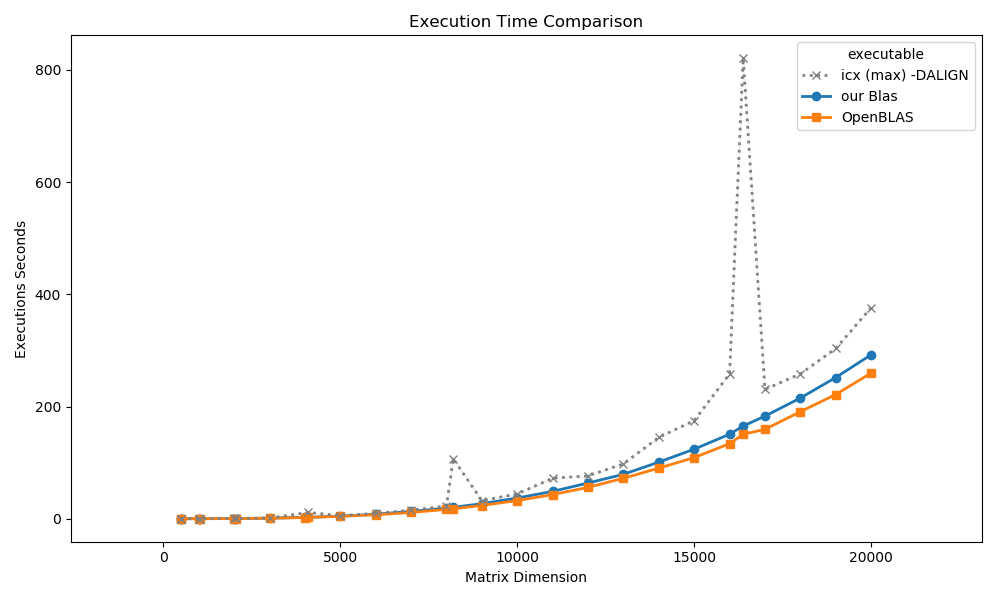
\includegraphics[width=0.8\textwidth]{Images/blas_vs_openblas.png}
\caption{Performance comparison of the original \texttt{OpenBLAS} and our custom implementation 
}
\label{fig:blas_vs_openblas}
\end{figure}

The plot clearly shows a smooth, cubic trends that \emph{finally} matches the suggested complexity of $O(n^3)$, and the already discussed  supremacy of the original version. 

We can now consider completed the quest of the search for the best possible sequential implementation.








% ========================================================================================
% ==================================COMPILER COMPARISON===================================
% ========================================================================================
\subsection{Final Comparison}
As illustrated in Figure~\ref{fig:all_seq_5000}, the in-depth study and progressive refinement of each version yields a consistently faster executable. 

\begin{figure}[H]
\centering
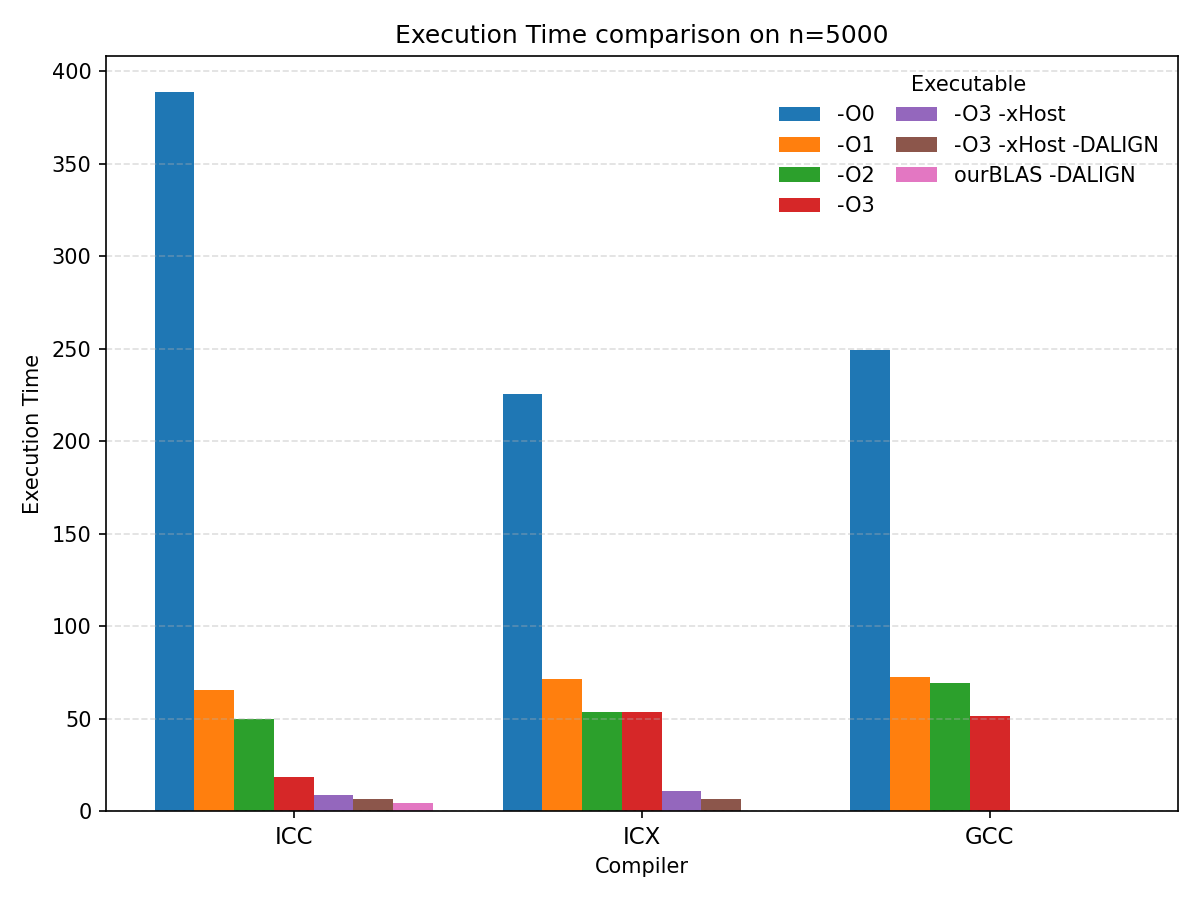
\includegraphics[width=0.8\textwidth]{Images/all_5000.png}
\caption{Comparison of all the previously proposed implementations for $N=5000$.}
\label{fig:all_seq_5000}
\end{figure}

The transition from naive memory accesses to compiler-driven tiling, and finally to explicit SIMD micro-kernels, effectively demonstrates the layers of optimization required to saturate modern hardware.

For the sake of completeness, we ultimately compare our best implementations against the absolute state-of-the-art for Dense Matrix Multiplication on our specific architecture: the \textbf{Intel Math Kernel Library (MKL)}\footnote{Intel MKL (now part of oneAPI) is a highly optimized, proprietary math library developed directly by Intel. It relies on hand-tuned assembly, hardware-specific prefetching, and undocumented architectural features to reach the absolute theoretical peak throughput of Intel processors.}. 

\input{Tables/sequential_comparison}

By treating the Intel MKL performance as our 100\% baseline, we can accurately quantify how each of our iterative versions approaches the hardware's maximum potential across different matrix dimensions. 

Using the GFLOPS computation formula detailed in Section~\ref{subsubsec:metrics}, we demonstrate that our custom implementation successfully achieves approximately \textbf{87\%} of the state-of-the-art peak performance.